%%%%%%%%%%%%%%%%%%%%%%%%%%%%%%%%%%%%%%%%%%%%%%%%
%% Compile the master file!
%% 		Slides: Antonio Machicao y Priemer
%% 		Course: GK Linguistik
%%%%%%%%%%%%%%%%%%%%%%%%%%%%%%%%%%%%%%%%%%%%%%%%


%%%%%%%%%%%%%%%%%%%%%%%%%%%%%%%%%%%%%%%%%%%%%%%%%%%%
%%%             Metadata                         
%%%%%%%%%%%%%%%%%%%%%%%%%%%%%%%%%%%%%%%%%%%%%%%%%%%%      

\title{Grundkurs Linguistik}

\subtitle{Sprache \& Sprachwissenschaft II}

\author[aMyP]{
	{\small Antonio Machicao y Priemer}
	\\
	{\footnotesize \url{http://www.linguistik.hu-berlin.de/staff/amyp}}
	%	\\
	%	\href{mailto:mapriema@hu-berlin.de}{mapriema@hu-berlin.de}}
}

\institute{Institut für deutsche Sprache und Linguistik}

\date{ }

%\publishers{\textbf{6. linguistischer Methodenworkshop \\ Humboldt-Universität zu Berlin}}

%\hyphenation{nobreak}


%%%%%%%%%%%%%%%%%%%%%%%%%%%%%%%%%%%%%%%%%%%%%%%%%%%%
%%%             Preamble's End                   
%%%%%%%%%%%%%%%%%%%%%%%%%%%%%%%%%%%%%%%%%%%%%%%%%%%%       


%%%%%%%%%%%%%%%%%%%%%%%%%      
\huberlintitlepage

\iftoggle{toc}{
\frame{
\begin{multicols}{2}
	\frametitle{Inhaltsverzeichnis}\tableofcontents
	%[pausesections]
\end{multicols}
	}
	}

%%%%%%%%%%%%%%%%%%%%%%%%%%%%%%%%%%
%%%%%%%%%%%%%%%%%%%%%%%%%%%%%%%%%%
%%%%%LITERATURE:

%% Allgemein
\nocite{Glueck&Roedel16a}
\nocite{Schierholz&Co18}
\nocite{Luedeling2009}
\nocite{Meibauer&Co07a} 
\nocite{Repp&Co15a} 


%%%%%%%%%%%%%%%%%%%%%%%%%%%%%%%%%%%
%%%%%%%%%%%%%%%%%%%%%%%%%%%%%%%%%%%
\section{Sprache \& Sprachwissenschaft II}
	
	
%%%%%%%%%%%%%%%%%%%%%%%%%%%%%%%%%%%
%%%%%%%%%%%%%%%%%%%%%%%%%%%%%%%%%%%
\subsection{Grammatik}
%\frame{
%\begin{multicols}{2}
%\frametitle{~}
%	\tableofcontents[currentsection]
%\end{multicols}
%}
%%%%%%%%%%%%%%%%%%%%%%%%%%%%%%%%%%%
	
\begin{frame}{Grammatik}
	\begin{itemize}
		\item Komplexität des Sprachsystems (Einheiten + Regeln) ist den Sprechern meist \textbf{nicht bewusst}.
		\item[]
		\item Die Linguistik interessiert sich für das unbewusste, internalisierte System $\rightarrow$ sprachliche \textbf{Kompetenz} der Sprecher
		\item[]
		\item Diese Kompetenz bildet die Grammatik einer Sprache.
	\end{itemize}
	
	\begin{block}<2->{Grammatik}
		System, das Laute und Bedeutungen \textbf{regelhaft einander zuordnet} und das gesamte Regelsystem einer Sprache umfasst.
	\end{block}	
\end{frame}


%%%%%%%%%%%%%%%%%%%%%%%%%%%%%%%%%%%
%%%%%%%%%%%%%%%%%%%%%%%%%%%%%%%%%%%
\subsubsection{Grammatikbegriff}
%\frame{
%\begin{multicols}{2}
%\frametitle{~}
%	\tableofcontents[currentsection]
%\end{multicols}
%}
%%%%%%%%%%%%%%%%%%%%%%%%%%%%%%%%%%%

\begin{frame}{Grammatikbegriff}

\begin{itemize}
	\item<1-> Grammatik im engeren Sinne als \textbf{Lehre} von morphologischen und syntaktischen Regularitäten einer Sprache. Unter dieser Auffassung bleiben die Phonologie und die Semantik als Teilbereiche der Sprachwissenschaft ausgeklammert (traditionelle Definition).
	\item[]
	\item<2-> Grammatik als \textbf{präskriptive/normative} Grammatik, die Vorgaben für die \gqq{korrekte} Sprachverwendung einer einzelnen Sprache (\gqq{gutes Deutsch}) macht (z.~B. \citet{DudenGramm09d}).
	\item[]
	\item<3-> Grammatik als \textbf{deskriptive} Grammatik, die eine wertungsfreie Beschreibung einer einzelnen Sprache gibt (z.~B. \citet{Eisenberg00a}, auch \gqq{Problemgrammatik} genannt).
\end{itemize}

\end{frame}


%%%%%%%%%%%%%%%%%%%%%%%%%%%%%%%%%%%
\begin{frame}

\begin{itemize}
	\item<1-> Grammatik als \textbf{Lehrbuch} oder \textbf{Nachschlagewerk}
	\item[]
	\item<2-> Grammatik für den Fremdsprachenunterricht (z.~B. \citet{Helbig&Buscha05a})
	\item[]
	\item<3-> Grammatik als \textbf{Sprachtheorie} (z.~B. Generative Grammatik (vgl. \citet{Philippi&Tewes10a}) oder Dependenzgrammatik (vgl. \citet{Agel00a}))
	\item[]
	\item<4-> In diesem Seminar verstehen wir Grammatik als:

	\begin{itemize}
		\item<4-> System, das Laute und Bedeutungen regelhaft einander zuordnet und das gesamte Regelsystem einer Sprache umfasst.
		\item<4-> Wir befassen uns mit Grammatik mit einer \textbf{deskriptiven} Methodik
                  (d.\,h. nicht präskriptiv!) und verwenden dafür (bzw. bilden dadurch)
                  \textbf{Grammatiktheorien}\\
(z.\,B. Generative Grammatik).
	\end{itemize}

\end{itemize}

\end{frame}


%%%%%%%%%%%%%%%%%%%%%%%%%%%%%%%%%%%
%%%%%%%%%%%%%%%%%%%%%%%%%%%%%%%%%%%
\subsubsection{Modularität der Grammatik}
%\frame{
%\begin{multicols}{2}
%\frametitle{~}
%	\tableofcontents[currentsection]
%\end{multicols}
%}
%%%%%%%%%%%%%%%%%%%%%%%%%%%%%%%%%%%

\begin{frame}{Modularität der Grammatik}
	
\begin{itemize}
	\item Hauptsächlich in der Generativen Grammatik angenommen (in anderen Grammatiktheorietraditionen umstritten)
	\item[]
	\item Sprachvermögen $\rightarrow$ modular organisiert
	\item<2-> Grammatik (oder die Sprache) ist ein \textbf{Modul} im \textbf{menschlichen kognitiven System}.
	\item<2-> Dieses (Sprach)modul besteht zugleich aus \textbf{miteinander interagierenden Teilmodulen} (sprachlichen Teilmodulen, grammatischen Ebenen oder sprachlichen Komponenten)
	\item[]
	\item<3-> Wie \textbf{selbstständig} diese Module sind, ist umstritten.
	\item[]
	\item<3-> Die \textbf{Evidenz} für diese Modularisierung findet die Generative Grammatik in der Aphasie-, Versprecher- und Spracherwerbsforschung.  
\end{itemize}

\end{frame}


%%%%%%%%%%%%%%%%%%%%%%%%%%%%%%%%%%%
\begin{frame}

\begin{itemize}
	\item Folgende Module werden angenommen (vgl. \citet{Abramowski2016}):
		
	\begin{itemize}
		\item[]
		\item Lexikon
		\item[]
		\item Phonologische Komponente
		\item[]
		\item Morphologische Komponente
		\item[]
		\item Syntaktische Komponente
		\item[]
		\item Semantische Komponente
		\item[]
	\end{itemize}
		
	\item<2-> Jedes sprachliche Modul besteht zugleich aus:
	
	\begin{enumerate}
		\item<2-> einem Inventar von komponentenspezifisch kategorisierten
                  \textbf{Minimaleinheiten}\\
                         (z.~B. Morphem in der Morphologie)
		\item<2->[] und
		\item<2-> einer Menge von komponentenspezifischen \textbf{Regeln zur Kombination} dieser Minimaleinheiten zu wohlgeformten komplexen Einheiten. 
	\end{enumerate}		  
		
\end{itemize}

\end{frame}


%%%%%%%%%%%%%%%%%%%%%%%%%%%%%%%%%%%
%%%%%%%%%%%%%%%%%%%%%%%%%%%%%%%%%%%
\subsubsubsection{Lexikon}

%\iftoggle{toc}{
%	\frame{
%		%\begin{multicols}{2}
%		\tableofcontents[currentsection]
%		%\end{multicols}
%	}
%}
%%%%%%%%%%%%%%%%%%%%%%%%%%%%%%%%%%%

\begin{frame}{Lexikon}
	
	\begin{itemize}
		\item \textbf{Repräsentation von Wörtern} und Wortteilen einer Sprache mit der \textbf{Information} über deren:

		\begin{enumerate}
			\item[]
			\item Aussprache (phonologische Information)
			\item[]
			\item interne Struktur (morphologische Information)
			\item[]
			\item syntaktische Kategorie und syntaktisches Kombinationspotential (syntaktische Information)
			\item[]
			\item Bedeutung (semantische Information) 
		\end{enumerate}		  
			
	\end{itemize}
		
\end{frame}


%%%%%%%%%%%%%%%%%%%%%%%%%%%%%%%%%%%
\begin{frame}{Lexikon}
			
\begin{itemize}
	\item Eintrag: \ab{\textsc{geb(en)}}

	\begin{enumerate}
		\item[]
		\item Phonologische Information: \textipa{/ge\textlengthmark{}b\textschwa{}n/}
		\item[]
		\item Morphologische Information: [[\ab{geb}] + [\ab{en}]]
		\item[]
		\item Syntaktische Information: \gqq{Ditransitives Verb}\\
%			\textsc{
%			NP_{1\{\textsc{nom}\}}+
%			NP_{2\{\textsc{dat}\}}+
%			NP_{3\{\textsc{akk}\}}+
%			V
%			}\\
%					
%		\item[]
%		\item Semantische Information:\\
%			\textsc{
%			NP_{1\{\textsc{agens}\}}+
%			NP_{2\{\textsc{goal}\}}+
%			NP_{3\{\textsc{thema}\}}+
%			V}\\
%			$\approx$\\
%			{[}\textsc{NP}_{1} \textsc{verursacht} {[}\textsc{NP}_{2} \textsc{erhält} \textsc{NP}_{3}]] 
	\end{enumerate}		  

\end{itemize}

\end{frame}


%%%%%%%%%%%%%%%%%%%%%%%%%%%%%%%%%%%
%%%%%%%%%%%%%%%%%%%%%%%%%%%%%%%%%%%
\subsubsubsection{Phonologische Komponente}

%\iftoggle{toc}{
%	\frame{
%		%\begin{multicols}{2}
%		\tableofcontents[currentsection]
%		%\end{multicols}
%	}
%}
%%%%%%%%%%%%%%%%%%%%%%%%%%%%%%%%%%%

\begin{frame}{Phonologische Komponente}

	\begin{itemize}
		\item Sie beschränkt das \textbf{Lautinventar} einer Sprache.
		\item[]
		\item Sie regelt die \textbf{Lautkombinatorik} und -veränderung.
		\item[]
		\item Festlegung von \textbf{Wort-} und \textbf{Satzakzent}

		\begin{itemize}
			\item[]
			\item<2->[$\rightarrow$] Wieso spricht man \ab{Hund} mit \textipa{[t]} aber \ab{Hunde} mit \textipa{[d]} aus?
			\item[]
			\item<3->[$\rightarrow$] Kann ein Wort im Deutschen mit der Lautfolge \textipa{[Ng]} beginnen?
			\item[]
			\item<4->[$\rightarrow$] Was ist der Unterschied zwischen \abu{HAUStürgriff} und \abu{HausTÜRgriff}?
		\end{itemize}		  
	
	\end{itemize}
	
\end{frame}


%%%%%%%%%%%%%%%%%%%%%%%%%%%%%%%%%%%
%%%%%%%%%%%%%%%%%%%%%%%%%%%%%%%%%%%
\subsubsubsection{Morphologische Komponente}

%%%%%%%%%%%%%%%%%%%%%%%%%%%%%%%%%%%

\begin{frame}{Morphologische Komponente}

\begin{itemize}
	\item Sie regelt die \textbf{interne Struktur von Wörtern}.
	\item[]
	\item Bildung von neuen Wörtern und Wortformen
				
	\begin{itemize}
		\item[]
		\item<2->[$\rightarrow$] Wie hängen \ab{kaufen} und \ab{kaufbar} zusammen?
		\item[]
		\item<3->[$\rightarrow$] Was zeigt \ab{-st} bei der Bildung neuer Verbformen an?
	\end{itemize}
			
\end{itemize}

\end{frame}


%%%%%%%%%%%%%%%%%%%%%%%%%%%%%%%%%%%
\begin{frame}{Morphologische Komponente}

\begin{itemize}
	\item[]
			
	\begin{itemize}
		\item[]
		\item[$\rightarrow$] Warum ist die eine Struktur des Wortes \ab{Bedeutungsableitung} intuitiv nicht korrekt und die andere schon?
	\end{itemize}
			
\end{itemize}

	
\begin{figure}[b]
	
	\begin{minipage}[b]{0.37\textwidth}
					\tiny{
		\begin{forest}MyP edges
		[Bedeutungsableitung [Be][deutungsableitung [deut][ungsableitung [ungsableit [ung][sableit [sab [s][ab]][leit]]][ung]]]]
		\end{forest}}
		
	\caption{Ungrammatisch}
	\end{minipage}
	%
	\begin{minipage}[b]{0.20\textwidth}
  	%	
	\end{minipage}
	%				
	\begin{minipage}[b]{0.37\textwidth}
	\tiny{
		\begin{forest}MyP edges
		[Bedeutungsableitung [Bedeutungs [Bedeutung [Bedeut [Be][deut]][ung]][s]][ableitung [ableit [ab][leit]][ung]]]
		\end{forest}}
			
	\caption{Grammatisch}
	\end{minipage}
	                        
\end{figure}

\end{frame}


%%%%%%%%%%%%%%%%%%%%%%%%%%%%%%%%%%%
%%%%%%%%%%%%%%%%%%%%%%%%%%%%%%%%%%%
\subsubsubsection{Syntaktische Komponente}

%%%%%%%%%%%%%%%%%%%%%%%%%%%%%%%%%%%
	
\begin{frame}{Syntaktische Komponente}

\begin{itemize}
	\item Sie regelt die \textbf{Struktur} von \textbf{Phrasen und Sätzen}.

	\begin{enumerate}
		\item[]
		\item<2->[$\rightarrow$] Wieso ist die Phrase (\ref{ex1a}) grammatisch und die Phrase (\ref{ex1b}) nicht?
		
\eal
	\ex \label{ex1a} Die Königin von Schweden aus Deutschland 
	\ex \label{ex1b} Die Königin aus Deutschland von Schweden
	\zl
		\item<3->[$\rightarrow$] Warum ist ein Satz wie (\ref{ex2a}) ungrammatisch (trotz alphabetischer Anordnung der Wörter), während (\ref{ex2b}) grammatisch ist?

\eal
	\ex[*]{Buch Chomsky das ich kaufen morgen von werde.}\label{ex2a}
	\ex[]{Das Buch von Chomsky werde ich morgen kaufen.}\label{ex2b}
	\zl
	
		\item<4->[$\rightarrow$] Aus welchem Grund hat der Satz unter (\ref{ex3}) zwei Bedeutungen? 

\ea Maria hat Peter geschlagen.\label{ex3}
\z

	\end{enumerate}
			
\end{itemize}

\end{frame}


%%%%%%%%%%%%%%%%%%%%%%%%%%%%%%%%%%%
%%%%%%%%%%%%%%%%%%%%%%%%%%%%%%%%%%%
\subsubsubsection{Semantische Komponente}

%%%%%%%%%%%%%%%%%%%%%%%%%%%%%%%%%%%
		
\begin{frame}{Semantische Komponente}
	
	\begin{itemize}
		\item Sie regelt die \textbf{Bedeutungsherleitung} komplexerer Einheiten (komplexer Wörter, Phrasen und Sätze).
		\item[]
		\item<2-> Wichtig bei der Herleitung $\rightarrow$ \textbf{Bedeutung der Bestandteile + Bedeutung der Struktur} (Kompositionalitäts- oder \textbf{Fregeprinzip})
				
		\begin{enumerate}
			\item<3->[$\rightarrow$] Worin besteht der Bedeutungsunterschied zwischen den Verben \ab{arbeiten} und \ab{bearbeiten}?
			\item<4->[$\rightarrow$] Wieso haben die Sätze (\ref{ex4a}) und (\ref{ex4b})
                          nicht die gleiche Bedeutung,\\
wenn sie aus den gleichen Wörtern bestehen?

\eal	
	\ex Maria hat Peter gesehen. \label{ex4a}
	\ex Hat Maria Peter gesehen? \label{ex4b}
\zl

			\item<5->[$\rightarrow$] Warum bedeutet \ab{sich} in (\ref{ex5a}) und (\ref{ex5b}) nicht dasselbe?
	
\eal
	\ex Maria verspricht sich, Mario zu treffen. \label{ex5a}
	\ex Maria verspricht Mario, sich zu treffen. \label{ex5b}
\zl

		\end{enumerate}
		
	\end{itemize}
	
\end{frame}


%%%%%%%%%%%%%%%%%%%%%%%%%%%%%%%%%%%
%%%%%%%%%%%%%%%%%%%%%%%%%%%%%%%%%%%
\subsubsubsection{Architektur des Sprachsystems}

%%%%%%%%%%%%%%%%%%%%%%%%%%%%%%%%%%%
		
\begin{frame}{Architektur des Sprachsystems}
	
	\begin{itemize}
		\item Sprachliche Strukturbildung wird durch die bereits erwähnten Komponenten geregelt.
		\item[]
		\item<2-> Außerdem interagiert das grammatische System der Sprache mit den folgenden \textbf{außersprachlichen Ebenen}:
				
		\begin{itemize}
			\item[]
			\item<3-> dem \textbf{artikulatorisch-perzeptorischen Apparat} (den biologischen Gegebenheiten zur Produktion und Rezeption von Sprachlauten)
			\item[]
			\item<3->[] und
			\item[]
			\item<4-> dem \textbf{konzeptuell-intentionalen System}, d.\,h. dem Bereich der Kognition, der sich mit Bedeutung befasst. Das konzeptuell-intentionale System wird wiederum durch Weltwissen, Kontextwissen und analytisches Wissen gespeist.
		\end{itemize}
			
	\end{itemize}
		
\end{frame}


%%%%%%%%%%%%%%%%%%%%%%%%%%%%%%%%%%%
%\begin{frame}{Architektur des Sprachsystems}

%\begin{figure}[H]
%\centering
				
%	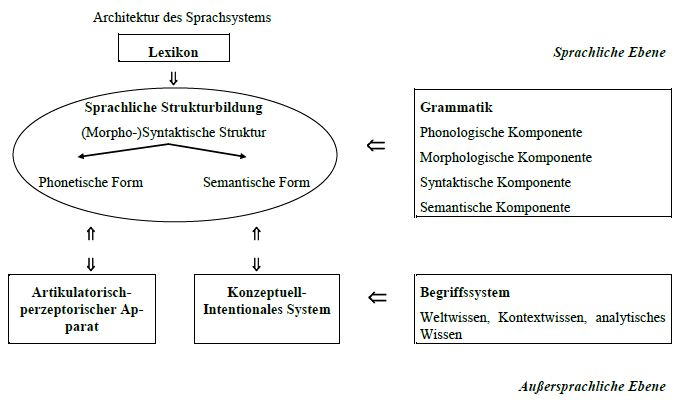
\includegraphics[width=\textwidth]{material/03ArchitekturSprachsystem.jpg}
%	\caption{Architektur des Sprachsystems \citep{Abramowski2016}}
%	\label{Zeichen3}

%\end{figure}

%\end{frame}			


%%%%%%%%%%%%%%%%%%%%%%%%%%%%%%%%%%%
\begin{frame}

\begin{figure}
\centering
\small
\begin{minipage}{0.55\textwidth}
\centering
\fbox{Lexikon}\\
\Large
$ \Downarrow $
\end{minipage}
%
\begin{minipage}{0.1\textwidth}
\centering
\hfill
\end{minipage}
%
\begin{minipage}[t]{0.3\textwidth}
\centering
\textit{Sprachliche Ebene}
\end{minipage}

\begin{minipage}[t]{0.55\textwidth}
\centering
\outputbox{\centering Sprachliche Strukturbildung\\
\begin{forest}sm edges,
[(Morpho-)Syntaktische Struktur
[Phonetische Form]
[Semantische Form]
]
\end{forest}}
\begin{tabular}{cp{3cm}c}
\Large
$ \Updownarrow $ && \Large $ \Updownarrow $\\
\end{tabular}
\end{minipage}
%
\begin{minipage}[c]{0.1\textwidth}
\centering
\Large
$ \Leftarrow $
\end{minipage}
%
\begin{minipage}[t]{0.3\textwidth}
\centering
\small
\outputbox{
Grammatik
\begin{itemize}
\item Phonologische Komponente\\
\item Morphologische K.\\
\item Syntaktische K.\\
\item Semantische K.
\end{itemize}}
\end{minipage}

\begin{minipage}{0.24\textwidth}
\centering
\outputbox{\centering Artikularisch-perzeptorischer Apparat}
\end{minipage}
%
\begin{minipage}[c]{0.05\textwidth}
\hfill
\end{minipage}
%
\begin{minipage}{0.24\textwidth}
\centering
\outputbox{\centering Konzeptuell-Intentionales System}
\end{minipage}
%
\begin{minipage}{0.1\textwidth}
\centering
\Large
$\Leftarrow$
\end{minipage}
%
\begin{minipage}{0.3\textwidth}
\outputbox{Begriffssystem
\newline
\small
Weltwissen, Kontextwissen, analytisches Wissen}
\end{minipage}

\begin{minipage}{0.65\textwidth}
\hfill
\end{minipage}
%
\begin{minipage}{0.3\textwidth}
\centering
\small
\textit{Außersprachliche Ebene}
\end{minipage}
\caption{Die Architektur des Sprachsystems \citep[vgl.]{Abramowski2016}}
\end{figure}

\end{frame}

%%%%%%%%%%%%%%%%%%%%%%%%%%%%%%%%%%%
%%%%%%%%%%%%%%%%%%%%%%%%%%%%%%%%%%%
\subsection{Linguistische Teildisziplinen}		

\iftoggle{toc}{
\frame{
\begin{multicols}{2}
	\tableofcontents[currentsection]
\end{multicols}
}
}
%%%%%%%%%%%%%%%%%%%%%%%%%%%%%%%%%%%

\begin{frame}{Linguistische Teildisziplinen}

	\begin{itemize}
		\item Phonologie
		\item Morphologie
		\item Syntax
		\item Semantik
		\item[]
		\item Phonetik
		\item Graphematik
		\item Pragmatik
		\item[]
		\item Psycholinguistik
		\item Soziolinguistik
		\item Historische Linguistik
		\item Korpuslinguistik
		\item \dots
	\end{itemize}
	
\end{frame}



%%%%%%%%%%%%%%%%%%%%%%%%%%%%%%%%%%%
%%%%%%%%%%%%%%%%%%%%%%%%%%%%%%%%%%%
\subsection{Linguistik als Geistes- und/oder Naturwissenschaft}		

\iftoggle{toc}{
\frame{
\begin{multicols}{2}
	\tableofcontents[currentsection]
\end{multicols}
}
}
%%%%%%%%%%%%%%%%%%%%%%%%%%%%%%%%%%%

\begin{frame}{Linguistik als Geistes- und/oder Naturwissenschaft}

	\begin{itemize}
		\item \textbf{Geisteswissenschaft}
		
		\begin{itemize}
			\item Verstehen von individuellen Leistungen des Geistes (eines Menschen, einer Gemeinschaft, einer Epoche)
			\item Verstehen von kulturellen Beziehungen und Entwicklungen
			\item[$\rightarrow$] Methode: \textbf{Hermeneutik} (Annähern durch Verstehen)
		\end{itemize}
		
		\item[]
		\item \textbf{Naturwissenschaft}
		
		\begin{itemize}
			\item Erklärung von naturgesetzlichen Kausalitäten und Zusammenhängen
			\item[$\rightarrow$] Methode: \textbf{Experiment}
		\end{itemize}
		
%		\item[]
%		\item Linguistik eher naturwissenschaftlich ausgerichtet (im Gegensatz zur Literaturwissenschaft)
	\end{itemize}
%%auch auf Folgefolie
	
\end{frame}		


%%%%%%%%%%%%%%%%%%%%%%%%%%%%%%%%%%%
\begin{frame}

	\begin{itemize}
		\item Linguistik \textit{eher} naturwissenschaftlich ausgerichtet (im Gegensatz zur Literaturwissenschaft)
		
		\begin{itemize}
			\item[]
			\item \textbf{Beobachtung} und \textbf{Analyse} von Gesetzen natürlicher Sprachen mit dem Ziel ihre \textbf{Systematik} aufzudecken (z.~B. Syntax)
			\item[]
			\item<2-> Arbeit mit \textbf{empirischen} Verfahren wie Experimenten (\zB Psycholinguistik) oder wie Ansammlungen von Daten (\zB Korpuslinguistik)) als Evidenz $\rightarrow$ \textbf{Naturwissenschaft}
			\item[]
			\item<3-> Beschäftigung mit der \textbf{Geschichte} einer Sprache (\zB Historische Linguistik) und mit den \textbf{sozialen} und kulturellen Bedingungen vom Sprachwandel (\zB Soziolinguistik) $\rightarrow$ \textbf{Geisteswissenschaft}
			\item[]
			\item<4-> Untersuchung des vielleicht \textbf{zentralsten Outputs des Geistes}: der Sprache (vgl. \citet{Meibauer&Co07a})
		\end{itemize}
		
	\end{itemize}
	
\end{frame}		


%%%%%%%%%%%%%%%%%%%%%%%%%%%%%%%%%%%
%%%%%%%%%%%%%%%%%%%%%%%%%%%%%%%%%%%
\subsection{Sprachwissenschaft vs. Linguistik}
\iftoggle{toc}{
\frame{
\begin{multicols}{2}
	\tableofcontents[currentsection]
\end{multicols}
}
}
%%%%%%%%%%%%%%%%%%%%%%%%%%%%%%%%%%%

\begin{frame}{Sprachwissenschaft vs. Linguistik}

	\begin{itemize}
		\item<1-> Linguistik und Sprachwissenschaft \idR \textbf{synonymisch} gebraucht
		\item[]
		\item<2-> Unterscheidung:
		
		\begin{itemize}
			\item[]
			\item<2-> Linguistik als \textbf{Teildisziplin} der Sprachwissenschaft
			\item[]
			\item<3-> \gqq{\textbf{Innere Sprachwissenschaft}} $\approx$ Linguistik $\rightarrow$ Beschäftigung mit innersprachlichen Sachverhalten und Entwicklungen (Sprache als System)
			\item[]
			\item<4-> \gqq{\textbf{Äußere Sprachwissenschaft}} $\rightarrow$ Beschäftigung mit kulturellen, sozialen, ökonomischen, politischen, usw. Bedingungen der Existenz und der Geschichte von Sprache, d.\,h. den äußeren (auch \textit{außersprachlich} genannten) Faktoren (vgl. \citet{Glueck05a})
		\end{itemize}
		
		\item[]
		\item<5-> In diesem Kurs werden wir jedoch beide Begriffe \textbf{gleichbedeutend} verwenden.
	\end{itemize}
	
\end{frame}

%%%%%%%%%%%%%%%%%%%%%%%%%%%%%%%%%%%


